\documentclass[10pt,a4paper]{article}
\usepackage[utf8]{inputenc}
\usepackage[T1]{fontenc}
\usepackage[romanian]{babel}
\usepackage[margin=1.7cm]{geometry}
\usepackage{amsmath,amssymb}
\usepackage{enumitem}
\usepackage{titlesec}
\usepackage{parskip}
\usepackage{tikz}
\usepackage{circuitikz}
\usepackage{pgfplots}
\pgfplotsset{compat=1.18}
\usetikzlibrary{arrows.meta}
\usepackage[most]{tcolorbox}
\newtcolorbox{keyeq}{colback=red!5,colframe=red!70!black,boxrule=0.7pt,arc=2pt,boxsep=2pt,left=5pt,right=5pt,top=3pt,bottom=3pt,boxsep=1pt}
\setlist{nosep, topsep=2pt, itemsep=2pt, leftmargin=1.4em}
\titlespacing*{\section}{0pt}{8pt}{4pt}
\titlespacing*{\subsection}{0pt}{6pt}{2pt}
\renewcommand{\baselinestretch}{0.97}
\pagestyle{plain}

\title{\vspace{-2cm}Rezumat examen PS (Prelucrarea Semnalelor)}
\author{}
\date{}

\begin{document}
\maketitle
\vspace{-1.2cm}

\section*{1. Semnale}
\textbf{Definiție:} Semnalul = mărime fizică cu proprietatea de a se propaga într-un mediu; conține un mesaj util + eventual perturbații. Matematic: $x:T\to M$ (în timp) sau $X:\Omega\to N$ (în frecvență).

\textbf{Clasificări:}
\begin{itemize}
\item după domeniul de definiție: \textbf{continue} (analogice, $T=\mathbb{R}$) vs \textbf{discrete} (eșantionate, $T=\mathbb{Z}$)
\item după nivelele de amplitudine: \textbf{continue în amplitudine} ($M$ infinită) vs \textbf{cuantificate} ($M$ finită; caz particular: semnal logic/binar cu 2 nivele)
\item după predictibilitate: \textbf{deterministe} (descrise analitic) vs \textbf{aleatoare/nedeterministe}
\end{itemize}

\textbf{Semnale deterministe} se împart în:
\begin{itemize}
\item \textbf{periodice}: armonice (SPA) și oarecare (SPO), cu $x(t)=x(t\pm nT)$
\item \textbf{neperiodice}: cvasi-periodice și tranzitorii/speciale
\end{itemize}

\textbf{Tipuri uzuale în automatică} (semnale tranzitorii speciale):
\begin{itemize}
\item impuls Dirac: $\delta(t)=\infty$ la $t=0$, $0$ altfel, $\int\delta(t)dt=1$; proprietate de filtrare $\int f(t)\delta(t-t_0)dt=f(t_0)$
\item treapta unitară: $1_+(t)=1$ pentru $t\ge0$, $0$ altfel; $\frac{d1_+(t)}{dt}=\delta(t)$
\item rampa unitară: $x(t)=t$ pentru $t\ge0$; $\frac{dx(t)}{dt}=1_+(t)$
\item semnalul armonic unitar: $x(t)=\sin\omega t$ pentru $t\ge0$, $0$ altfel
\end{itemize}

\textbf{Semnal armonic — definiție, notații:} $x(t)=A\sin(2\pi t/T)=A\sin(2\pi f_1 t)=A\sin(\omega_1 t)$. Complet caracterizat de amplitudine $A$ și pulsație $\omega_1$ (sau frecvență $f_1$, perioadă $T$); $\omega_1=2\pi/T=2\pi f_1$.

\section*{2. Metode de analiză a semnalelor}
\textbf{Enumerare metode:}
\begin{itemize}
\item descompunerea în serie Fourier (reală/complexă) — pentru semnale periodice (spectrul Fourier)
\item mediile temporale și funcțiile de corelație
\item tehnici de analiză funcțională: transformatele Laplace, Z și Fourier
\item funcțiile de densitate spectrală de putere
\end{itemize}

\textbf{Valori medii temporale:}
\begin{itemize}
\item ordinul I: $\overline{x(t)}=\lim_{T\to\infty}\frac{1}{T}\int_{-T/2}^{T/2}x(t)\,dt$ — reprezintă componenta continuă a semnalului
\item ordinul II (pătratică): $\overline{x^2(t)}=\lim_{T\to\infty}\frac{1}{T}\int_{-T/2}^{T/2}x^2(t)\,dt$ — reprezintă puterea semnalului (la încărcare unitară)
\item varianța: $\mathrm{var}(x)=\lim_{T\to\infty}\frac{1}{T}\int[x(t)-\overline{x(t)}]^2dt$ — media pătratică a semnalului centrat
\end{itemize}
Proprietate: media de ordinul I nu depinde de originea timpului.

\textbf{Funcții de corelație:}
\begin{itemize}
\item autocorelație: $R_{xx}(\tau)=\overline{x(t+\tau)x(t)}$ — pară ($R_{xx}(-\tau)=R_{xx}(\tau)$), $R_{xx}(0)=\overline{x^2(t)}$ (puterea)
\item intercorelație: $R_{yx}(\tau)=\overline{y(t+\tau)x(t)}$, cu $R_{xy}(-\tau)=R_{yx}(\tau)$
\end{itemize}

\textbf{Funcții de covarianță} = funcții de corelație calculate pe semnalele centrate $x_0(t)=x(t)-\overline{x(t)}$:
\begin{itemize}
\item autocovarianță: $C_{xx}(\tau)=\overline{x_0(t+\tau)x_0(t)}$; $C_{xx}(0)=\mathrm{var}(x)$
\item intercovarianță: $C_{yx}(\tau)=\overline{y_0(t+\tau)x_0(t)}$; $C_{yx}(0)=\mathrm{cov}(x,y)$
\end{itemize}

\section*{3. Transformata Fourier (directă și inversă)}
\textbf{Relații de definiție:}
\begin{keyeq}\color{red!65!black}
$$X(\omega)=\int_{-\infty}^{\infty}x(t)e^{-j\omega t}dt=\mathcal{F}\{x(t)\} \qquad x(t)=\frac{1}{2\pi}\int_{-\infty}^{\infty}X(\omega)e^{j\omega t}d\omega=\mathcal{F}^{-1}\{X(\omega)\}$$
\end{keyeq}
$X(\omega)=M_X(\omega)e^{-j\varphi_X(\omega)}$, perechea Fourier se notează $x(t)\Leftrightarrow X(\omega)$.

\textbf{Teorema (proprietatea) de dualitate:} dacă $x(t)\Leftrightarrow y(\omega)$, atunci
$$x(\omega)\Leftrightarrow \frac{1}{2\pi}y(-t) \quad\text{echivalent}\quad y(-t)\Leftrightarrow 2\pi x(\omega)$$
(se inversează reciproc $t$ cu $\omega$, respectiv mărimile constante $T$ cu $\Omega=2\pi/T$).

\textbf{Semnalul poartă temporală:}
\begin{itemize}
\item \emph{centrată}: $w_T^c(t)=1$ pentru $|t|\le T/2$, $0$ altfel $\;\Leftrightarrow\; W_T^c(\omega)=T\,\mathrm{sinc}\!\left(\frac{\omega T}{2}\right)=T\dfrac{\sin(\omega T/2)}{\omega T/2}$
\item \emph{necentrată}: $w_T(t)=1$ pentru $t\in[0,T]$, $0$ altfel $\;\Leftrightarrow\; W_T(\omega)=e^{-j\omega T/2}\,W_T^c(\omega)$ (teorema translației temporale)
\end{itemize}

\textbf{Ce reprezintă spectrul Fourier:} este reprezentarea semnalului în domeniul amplitudine–pulsație (frecvență), echivalentă cu reprezentarea temporală — descrie aceeași informație/fenomen fizic, dar arată cum se distribuie amplitudinea (modulul) și faza semnalului pe componentele de frecvență care îl alcătuiesc.

\section*{4. Filtre}
\textbf{Definiție:} sistem selectiv în frecvență — circuit care transmite la ieșire, nemodificat, un anumit spectru din semnalul de intrare, atenuând/eliminând restul componentelor de frecvență.

\textbf{Cele 4 tipuri de filtre ideale:}
\begin{enumerate}
\item trece-jos (TJ)
\item trece-sus (TS)
\item trece-bandă (TB)
\item oprește-bandă (OB)
\end{enumerate}

\textbf{Caracteristicile ideale ale filtrelor:}
\begin{itemize}
\item amplitudinea răspunsului $|G(j\omega)|$ este constantă (=1) în banda de trecere și exact $0$ în afara ei (tranziție bruscă, fără bandă de tranziție)
\item faza $\Psi(\omega)$ are variație liniară $\Psi(\omega)=-\omega t_d$ (cu $t_d\ge0$) în toată banda de trecere $\Rightarrow$ semnalul e transmis fără distorsiuni, doar întârziat cu $t_d$
\item filtrele ideale \textbf{nu sunt realizabile fizic} (cauzale) — răspunsul pondere $g(t)$ este nenul pentru $t<0$ (sistem necauzal); din acest motiv filtrele reale aproximează caracteristica ideală cu o bandă de tranziție finită
\end{itemize}

\begin{center}
\begin{minipage}{0.24\linewidth}\centering
\begin{tikzpicture}[scale=0.55]
\draw[->] (0,0) -- (4,0) node[right]{\tiny $\omega$};
\draw[->] (0,0) -- (0,1.6) node[above]{};
\draw[thick] (0,1) -- (2,1) -- (2,0) -- (4,0);
\node[below] at (2,0) {\tiny $\omega_c$};
\end{tikzpicture}\\ \scriptsize Trece-jos
\end{minipage}\hfill
\begin{minipage}{0.24\linewidth}\centering
\begin{tikzpicture}[scale=0.55]
\draw[->] (0,0) -- (4,0) node[right]{\tiny $\omega$};
\draw[->] (0,0) -- (0,1.6) node[above]{};
\draw[thick] (0,0) -- (2,0) -- (2,1) -- (4,1);
\node[below] at (2,0) {\tiny $\omega_c$};
\end{tikzpicture}\\ \scriptsize Trece-sus
\end{minipage}\hfill
\begin{minipage}{0.24\linewidth}\centering
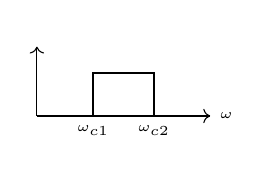
\begin{tikzpicture}[scale=0.55]
\draw[->] (0,0) -- (4,0) node[right]{\tiny $\omega$};
\draw[->] (0,0) -- (0,1.6) node[above]{};
\draw[thick] (0,0) -- (1.3,0) -- (1.3,1) -- (2.7,1) -- (2.7,0) -- (4,0);
\node[below] at (1.3,0) {\tiny $\omega_{c1}$};
\node[below] at (2.7,0) {\tiny $\omega_{c2}$};
\end{tikzpicture}\\ \scriptsize Trece-bandă
\end{minipage}\hfill
\begin{minipage}{0.24\linewidth}\centering
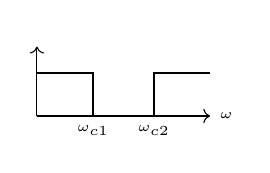
\begin{tikzpicture}[scale=0.55]
\draw[->] (0,0) -- (4,0) node[right]{\tiny $\omega$};
\draw[->] (0,0) -- (0,1.6) node[above]{};
\draw[thick] (0,1) -- (1.3,1) -- (1.3,0) -- (2.7,0) -- (2.7,1) -- (4,1);
\node[below] at (1.3,0) {\tiny $\omega_{c1}$};
\node[below] at (2.7,0) {\tiny $\omega_{c2}$};
\end{tikzpicture}\\ \scriptsize Oprește-bandă
\end{minipage}
\end{center}

\section*{5. Influența polilor și zerourilor asupra caracteristicii modul-pulsație}
\textbf{Funcția de transfer generală} (grade numărător = numitor): $G(s)=b_n\dfrac{(s-z_1)\dots(s-z_n)}{(s-\lambda_1)\dots(s-\lambda_n)}$, cu $z_i$ = zerouri, $\lambda_i$ = poli.

\textbf{Determinarea modulului — metoda geometrică:} un factor $(p-z)$ este un vector în planul complex, de la $z$ la $p$, cu modul $r=|p-z|$ și unghi $\varphi=\arg(p-z)$. Notând $r_i=|p-z_i|$ (distanțe de la zerouri la $p$) și $d_i=|p-\lambda_i|$ (distanțe de la poli la $p$):
\begin{keyeq}\color{red!65!black}
$$|G(s)|_{s=p}=|b_n|\,\dfrac{r_1r_2\dots r_n}{d_1d_2\dots d_n}=|b_n|\,\dfrac{\text{produsul distanțelor de la zerouri la }p}{\text{produsul distanțelor de la poli la }p}$$
\end{keyeq}
$$\angle G(s)|_{s=p}=(\varphi_1+\dots+\varphi_n)-(\theta_1+\dots+\theta_n)=\text{suma unghiurilor zerourilor}-\text{suma unghiurilor polilor}$$
Pentru răspunsul în frecvență se ia $p=j\omega$ și se variază $\omega\in(0,\infty)$.

\textbf{Influența unui pol} (caz $\lambda=-\alpha+j\omega_0$): notând $d$ = distanța de la pol la punctul curent $j\omega$, avem $|G(j\omega)|=k/d$. Pe măsură ce $\omega$ crește de la $0$ spre $\omega_0$, $d$ descrește $\Rightarrow$ câștigul \textbf{crește}; pentru $\omega>\omega_0$, $d$ crește $\Rightarrow$ câștigul \textbf{descrește}. Rezultă un \textbf{vârf de rezonanță} la $\omega_0$ (frecvența de rezonanță). Cât mai mic $\alpha$ (pol mai apropiat de axa $j\omega$), cu atât mai mare creșterea câștigului; la limită $\alpha=0$ (pol pe axa imaginară) câștigul la $\omega_0$ tinde la $\infty$. Polul conjugat $-\alpha-j\omega_0$ (perechile complexe apar mereu conjugate) nu modifică apreciabil efectul din vecinătatea lui $\omega_0$ (e relativ departe). Faza unei perechi de poli complecși conjugați variază de la $0$ (la $\omega=0$) la $-\pi$ (la $\omega\to\infty$).

\textbf{Influența unui zero} (caz $-\alpha\pm j\omega_0$): efect \textbf{opus} polului — \textbf{reduce} câștigul în vecinătatea lui $\omega_0$ (adâncitură/minim). Un zero exact pe axa imaginară ($\alpha=0$) produce câștig \textbf{nul} la $\omega_0$ (filtru "notch"). Zerouri multiple accentuează efectul. Faza unei perechi de zerouri complexe variază de la $0$ (la $\omega=0$) la $+\pi$ (la $\omega\to\infty$) — opus față de poli.

\textit{Aplicație — proiectare prin plasare poli/zerouri:} TJ $\Rightarrow$ pol(i) pe semiaxa reală negativă (câștig maxim la $\omega=0$); cu mai mulți poli pe un perete semicircular în SCS se obține familia \textbf{Butterworth}; TB $\Rightarrow$ poli plasați opuși axei imaginare în jurul lui $\pm\omega_0$; filtru \textbf{notch} (OB) de ordin 2 $\Rightarrow$ zerouri pe axa imaginară $\pm j\omega_0$ și poli pe semicercul de rază $\omega_0$, apropiați de zerouri (unghi $\theta\approx\pi/2$) pentru tranziție abruptă.

\textit{Proprietatea de complementaritate:} $G_{BS}(s)=1-G_{BP}(s)$ și $G_{LP}(s)=1-G_{HP}(s)$ (pentru filtre centrate/cu aceeași $\omega_0$, respectiv $\omega_c$).

\begin{center}
\begin{minipage}{0.48\linewidth}\centering
\scriptsize\textbf{Pol apropiat de axă $\Rightarrow$ vârf de rezonanță}\\[1mm]
\begin{tikzpicture}[scale=0.62]
\draw[->] (-2,0) -- (0.6,0) node[right]{\tiny Re};
\draw[->] (0,-1.2) -- (0,1.6) node[above]{\tiny Im};
\draw[dashed] (-1.4,1) -- (0,1);
\node at (-1.4,1) {\large $\times$};
\node[above left] at (-1.4,1) {\tiny $-\alpha\!+\!j\omega_0$};
\begin{scope}[xshift=4.4cm]
\draw[->] (0,0) -- (3.0,0) node[right]{\tiny $\omega$};
\draw[->] (0,0) -- (0,1.6) node[above]{\tiny $|G|$};
\draw[thick] (0,0.4) .. controls (0.9,0.5) and (1.2,1.5) .. (1.5,1.5) .. controls (1.8,1.5) and (2.1,0.5) .. (3.0,0.35);
\draw[dashed] (1.5,0) -- (1.5,1.5);
\node[below] at (1.5,0) {\tiny $\omega_0$};
\end{scope}
\end{tikzpicture}
\end{minipage}\hfill
\begin{minipage}{0.48\linewidth}\centering
\scriptsize\textbf{Zero pe axa $j\omega$ $\Rightarrow$ atenuare totală (notch)}\\[1mm]
\begin{tikzpicture}[scale=0.62]
\draw[->] (-2,0) -- (0.6,0) node[right]{\tiny Re};
\draw[->] (0,-1.2) -- (0,1.6) node[above]{\tiny Im};
\node at (0,1) {\Large $\circ$};
\node[left] at (0,1) {\tiny $j\omega_0$};
\begin{scope}[xshift=4.4cm]
\draw[->] (0,0) -- (3.0,0) node[right]{\tiny $\omega$};
\draw[->] (0,0) -- (0,1.6) node[above]{\tiny $|G|$};
\draw[thick] (0,1.3) .. controls (0.9,1.2) and (1.2,0.1) .. (1.5,0.05) .. controls (1.8,0.1) and (2.1,1.2) .. (3.0,1.3);
\draw[dashed] (1.5,0) -- (1.5,1.3);
\node[below] at (1.5,0) {\tiny $\omega_0$};
\end{scope}
\end{tikzpicture}
\end{minipage}
\end{center}

\section*{6. Specificațiile de proiectare ale filtrelor analogice}
Conceptele generale: \textbf{banda de trecere} = gama de frecvențe în care câștigul este cuprins între $1$ și $G_p$ ($G_p<1$, câștigul minim acceptat); \textbf{banda de oprire} = gama în care câștigul este sub valoarea $G_s$ (câștigul maxim admis); \textbf{banda de tranziție} = zona dintre ele — la filtrele reale tranziția e graduală (nu bruscă ca la cele ideale); condiția Paley-Wiener arată că nu poate exista câștig exact $0$ pe o bandă finită. Câștigul se exprimă în decibeli: $\hat{G}[\mathrm{dB}]=20\lg G$; atenuarea $\alpha=1/G$, $\hat\alpha[\mathrm{dB}]=-\hat G$.

\textbf{Specificul fiecărui tip de filtru} (pulsațiile de la $G_p$ se numesc $\omega_p$, cele de la $G_s$ se numesc $\omega_s$):
\begin{itemize}
\item \textbf{trece-jos (TJ)}: trecere pe $[0,\omega_p]$, oprire pe $[\omega_s,\infty)$, cu $\omega_p<\omega_s$
\item \textbf{trece-sus (TS)}: \textbf{invers} față de TJ — oprire pe $[0,\omega_s]$, trecere pe $[\omega_p,\infty)$, cu $\omega_s<\omega_p$
\item \textbf{trece-bandă (TB)}: oprire pe $[0,\omega_{s1}]\cup[\omega_{s2},\infty)$, trecere pe $[\omega_{p1},\omega_{p2}]$ (la mijloc), cu $\omega_{s1}<\omega_{p1}<\omega_{p2}<\omega_{s2}$
\item \textbf{oprește-bandă (OB)}: \textbf{invers} față de TB — trecere pe $[0,\omega_{p1}]\cup[\omega_{p2},\infty)$, oprire pe $[\omega_{s1},\omega_{s2}]$ (la mijloc), cu $\omega_{p1}<\omega_{s1}<\omega_{s2}<\omega_{p2}$
\end{itemize}

\begin{center}
\begin{minipage}{0.24\linewidth}\centering
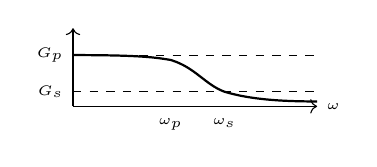
\begin{tikzpicture}[scale=0.62]
\draw[->] (0,0) -- (5,0) node[right]{\tiny $\omega$};
\draw[->] (0,0) -- (0,1.6);
\draw[dashed] (0,1.05) -- (5,1.05); \node[left] at (0,1.05) {\tiny $G_p$};
\draw[dashed] (0,0.3) -- (5,0.3); \node[left] at (0,0.3) {\tiny $G_s$};
\draw[thick] (0,1.05) .. controls (1.4,1.05) and (1.7,1.0) .. (2.0,0.95) .. controls (2.5,0.8) and (2.7,0.45) .. (3.1,0.3) .. controls (3.6,0.15) and (4.2,0.1) .. (5,0.1);
\node[below] at (2.0,-0.05) {\tiny $\omega_p$};
\node[below] at (3.1,-0.05) {\tiny $\omega_s$};
\end{tikzpicture}\\ \scriptsize Trece-jos
\end{minipage}\hfill
\begin{minipage}{0.24\linewidth}\centering
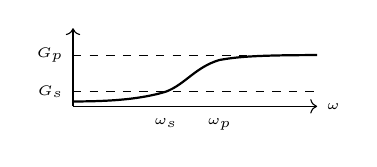
\begin{tikzpicture}[scale=0.62]
\draw[->] (0,0) -- (5,0) node[right]{\tiny $\omega$};
\draw[->] (0,0) -- (0,1.6);
\draw[dashed] (0,1.05) -- (5,1.05); \node[left] at (0,1.05) {\tiny $G_p$};
\draw[dashed] (0,0.3) -- (5,0.3); \node[left] at (0,0.3) {\tiny $G_s$};
\draw[thick] (0,0.1) .. controls (0.8,0.1) and (1.4,0.15) .. (1.9,0.3) .. controls (2.3,0.45) and (2.5,0.8) .. (3.0,0.95) .. controls (3.3,1.0) and (3.6,1.05) .. (5,1.05);
\node[below] at (1.9,-0.05) {\tiny $\omega_s$};
\node[below] at (3.0,-0.05) {\tiny $\omega_p$};
\end{tikzpicture}\\ \scriptsize Trece-sus
\end{minipage}\hfill
\begin{minipage}{0.24\linewidth}\centering
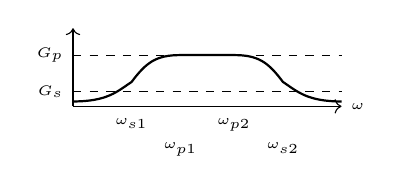
\begin{tikzpicture}[scale=0.62]
\draw[->] (0,0) -- (5.5,0) node[right]{\tiny $\omega$};
\draw[->] (0,0) -- (0,1.6);
\draw[dashed] (0,1.05) -- (5.5,1.05); \node[left] at (0,1.05) {\tiny $G_p$};
\draw[dashed] (0,0.3) -- (5.5,0.3); \node[left] at (0,0.3) {\tiny $G_s$};
\draw[thick] (0,0.1) .. controls (0.7,0.1) and (0.9,0.3) .. (1.2,0.5) .. controls (1.5,0.9) and (1.7,1.05) .. (2.2,1.05) -- (3.3,1.05) .. controls (3.8,1.05) and (4.0,0.9) .. (4.3,0.5) .. controls (4.6,0.3) and (4.8,0.1) .. (5.5,0.1);
\node[below] at (1.2,-0.05) {\tiny $\omega_{s1}$};
\node[below] at (2.2,-0.55) {\tiny $\omega_{p1}$};
\node[below] at (3.3,-0.05) {\tiny $\omega_{p2}$};
\node[below] at (4.3,-0.55) {\tiny $\omega_{s2}$};
\end{tikzpicture}\\ \scriptsize Trece-bandă
\end{minipage}\hfill
\begin{minipage}{0.24\linewidth}\centering
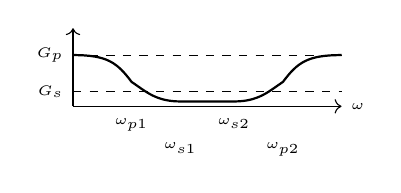
\begin{tikzpicture}[scale=0.62]
\draw[->] (0,0) -- (5.5,0) node[right]{\tiny $\omega$};
\draw[->] (0,0) -- (0,1.6);
\draw[dashed] (0,1.05) -- (5.5,1.05); \node[left] at (0,1.05) {\tiny $G_p$};
\draw[dashed] (0,0.3) -- (5.5,0.3); \node[left] at (0,0.3) {\tiny $G_s$};
\draw[thick] (0,1.05) .. controls (0.7,1.05) and (0.9,0.9) .. (1.2,0.5) .. controls (1.5,0.3) and (1.7,0.1) .. (2.2,0.1) -- (3.3,0.1) .. controls (3.8,0.1) and (4.0,0.3) .. (4.3,0.5) .. controls (4.6,0.9) and (4.8,1.05) .. (5.5,1.05);
\node[below] at (1.2,-0.05) {\tiny $\omega_{p1}$};
\node[below] at (2.2,-0.55) {\tiny $\omega_{s1}$};
\node[below] at (3.3,-0.05) {\tiny $\omega_{s2}$};
\node[below] at (4.3,-0.55) {\tiny $\omega_{p2}$};
\end{tikzpicture}\\ \scriptsize Oprește-bandă
\end{minipage}
\end{center}

\section*{7. Filtre RLC}
\textbf{Metodă generală:} se determină $H(s)=V_{out}(s)/V_{in}(s)$ printr-un divizor de tensiune cu impedanțe complexe ($Z_R=R$, $Z_L=sL$, $Z_C=1/(sC)$), apoi se identifică tipul de filtru observând comportarea lui $H(s)$ la $s\to0$ ($\omega=0$), $s\to\infty$ ($\omega\to\infty$) și la rezonanță $\omega_0=1/\sqrt{LC}$:
\begin{itemize}
\item $H(0)=1,\,H(\infty)=0$ (fără zerouri la numărător) $\Rightarrow$ \textbf{trece-jos}
\item $H(0)=0,\,H(\infty)=1$ $\Rightarrow$ \textbf{trece-sus}
\item $H(0)=0,\,H(\infty)=0$, maxim la $\omega_0$ $\Rightarrow$ \textbf{trece-bandă}
\item $H(0)=1,\,H(\infty)=1$, zero (minim total) la $\omega_0$ $\Rightarrow$ \textbf{oprește-bandă}
\end{itemize}

\textbf{Cele 8 scheme din tematică} (2 variante pentru fiecare tip de filtru):

\begin{center}
\begin{minipage}{0.24\linewidth}\centering
\begin{circuitikz}[scale=0.7, every node/.style={scale=0.8}]
\draw (0,1.5) to[R,l=$R$] (1.6,1.5) to[L,l=$L$] (3.2,1.5) -- (4.2,1.5);
\draw (3.2,1.5) to[C,l_=$C$] (3.2,0);
\draw (0,0) -- (4.2,0);
\end{circuitikz}\\ \scriptsize Trece-jos (a)
\end{minipage}\hfill
\begin{minipage}{0.24\linewidth}\centering
\begin{circuitikz}[scale=0.7, every node/.style={scale=0.8}]
\draw (0,1.5) to[R,l=$R$] (1.6,1.5) to[C,l=$C$] (3.2,1.5) -- (4.2,1.5);
\draw (3.2,1.5) to[L,l_=$L$] (3.2,0);
\draw (0,0) -- (4.2,0);
\end{circuitikz}\\ \scriptsize Trece-sus (b)
\end{minipage}\hfill
\begin{minipage}{0.24\linewidth}\centering
\begin{circuitikz}[scale=0.7, every node/.style={scale=0.8}]
\draw (0,1.5) to[L,l=$L$] (1.6,1.5) to[C,l=$C$] (3.2,1.5) -- (4.2,1.5);
\draw (3.2,1.5) to[R,l_=$R$] (3.2,0);
\draw (0,0) -- (4.2,0);
\end{circuitikz}\\ \scriptsize Trece-bandă (c)
\end{minipage}\hfill
\begin{minipage}{0.24\linewidth}\centering
\begin{circuitikz}[scale=0.7, every node/.style={scale=0.8}]
\draw (0,1.5) to[R,l=$R$] (1.9,1.5);
\draw (1.9,1.5) -- (2.9,1.5);
\draw (1.9,1.5) to[L,l_=$L$] (1.9,0);
\draw (2.9,1.5) to[C,l_=$C$] (2.9,0);
\draw (1.9,0) -- (2.9,0);
\draw (2.9,1.5) -- (4.2,1.5);
\draw (0,0) -- (4.2,0);
\end{circuitikz}\\ \scriptsize Oprește-bandă (d)
\end{minipage}

\vspace{5mm}

\begin{minipage}{0.24\linewidth}\centering
\begin{circuitikz}[scale=0.7, every node/.style={scale=0.8}]
\draw (0,1.5) to[L,l=$L$] (1.9,1.5);
\draw (1.9,1.5) -- (2.9,1.5);
\draw (1.9,1.5) to[C,l_=$C$] (1.9,0);
\draw (2.9,1.5) to[R,l_=$R$] (2.9,0);
\draw (1.9,0) -- (2.9,0);
\draw (2.9,1.5) -- (4.2,1.5);
\draw (0,0) -- (4.2,0);
\end{circuitikz}\\ \scriptsize Trece-jos (a)
\end{minipage}\hfill
\begin{minipage}{0.24\linewidth}\centering
\begin{circuitikz}[scale=0.7, every node/.style={scale=0.8}]
\draw (0,1.5) to[C,l=$C$] (1.9,1.5);
\draw (1.9,1.5) -- (2.9,1.5);
\draw (1.9,1.5) to[L,l_=$L$] (1.9,0);
\draw (2.9,1.5) to[R,l_=$R$] (2.9,0);
\draw (1.9,0) -- (2.9,0);
\draw (2.9,1.5) -- (4.2,1.5);
\draw (0,0) -- (4.2,0);
\end{circuitikz}\\ \scriptsize Trece-sus (b)
\end{minipage}\hfill
\begin{minipage}{0.24\linewidth}\centering
\begin{circuitikz}[scale=0.7, every node/.style={scale=0.8}]
\draw (0,1.5) to[R,l=$R$] (1.9,1.5);
\draw (1.9,1.5) -- (2.9,1.5);
\draw (1.9,1.5) to[C,l_=$C$] (1.9,0);
\draw (2.9,1.5) to[L,l_=$L$] (2.9,0);
\draw (1.9,0) -- (2.9,0);
\draw (2.9,1.5) -- (4.2,1.5);
\draw (0,0) -- (4.2,0);
\end{circuitikz}\\ \scriptsize Trece-bandă (c)
\end{minipage}\hfill
\begin{minipage}{0.24\linewidth}\centering
\begin{circuitikz}[scale=0.7, every node/.style={scale=0.8}]
\draw (0,1.5) -- (0.6,1.5);
\draw (0.6,1.5) to[L,l=$L$] (3.4,1.5);
\draw (0.6,1.0) to[C,l_=$C$] (3.4,1.0);
\draw (0.6,1.5) -- (0.6,1.0);
\draw (3.4,1.5) -- (3.4,1.0);
\draw (3.4,1.5) -- (4.2,1.5);
\draw (3.4,1.5) to[R,l_=$R$] (3.4,0);
\draw (0,0) -- (4.2,0);
\end{circuitikz}\\ \scriptsize Oprește-bandă (d)
\end{minipage}
\end{center}

\textbf{Exemple tipice (R,L serie + C shunt la ieșire, respectiv variante):}
\begin{keyeq}\color{red!65!black}
$$H_{TJ}(s)=\dfrac{1/(LC)}{s^2+\frac{R}{L}s+\frac{1}{LC}}\qquad H_{TS}(s)=\dfrac{s^2}{s^2+\frac{R}{L}s+\frac{1}{LC}}$$
$$H_{TB}(s)=\dfrac{\frac{R}{L}s}{s^2+\frac{R}{L}s+\frac{1}{LC}}\qquad H_{OB}(s)=\dfrac{s^2+\frac{1}{LC}}{s^2+\frac{R}{L}s+\frac{1}{LC}}$$
\end{keyeq}
toate de ordinul II, cu $\omega_0=1/\sqrt{LC}$ pulsația caracteristică (de rezonanță, respectiv de "notch" la OB). Pentru un circuit RLC concret dat la examen: se scriu impedanțele celor 2-3 ramuri, se aplică divizorul de tensiune, se simplifică la forma standard de mai sus și se compară cu cele 4 tipare ca să se identifice tipul.

\begin{center}
\begin{tikzpicture}
\begin{axis}[width=9.5cm,height=5.2cm,xlabel={\scriptsize $\omega$ (exemplu $L=C=R=1$)},ylabel={\scriptsize $|H(j\omega)|$},xmin=0,xmax=5,ymin=0,ymax=1.4,
  legend style={font=\tiny,at={(0.98,0.98)},anchor=north east},
  tick label style={font=\tiny}, label style={font=\scriptsize}]
\addplot[thick,blue] table {figdata/rlc_tj.dat}; \addlegendentry{TJ}
\addplot[thick,red] table {figdata/rlc_ts.dat}; \addlegendentry{TS}
\addplot[thick,green!50!black] table {figdata/rlc_tb.dat}; \addlegendentry{TB}
\addplot[thick,orange!90!black] table {figdata/rlc_ob.dat}; \addlegendentry{OB}
\end{axis}
\end{tikzpicture}
\end{center}

\textbf{Exemplu rezolvat} (circuitul trece-jos: $R,L$ serie $+$ $C$ shunt, vezi schema (a)): impedanțe $Z_R=R$, $Z_L=sL$, $Z_C=1/(sC)$; divizor de tensiune:
$$H(s)=\dfrac{Z_C}{R+sL+Z_C}=\dfrac{1/(sC)}{R+sL+1/(sC)}=\dfrac{1}{s^2LC+sRC+1}=\dfrac{1/(LC)}{s^2+\frac{R}{L}s+\frac{1}{LC}}$$
Numeric, cu $R=100\,\Omega$, $L=0{,}1$H, $C=1\,\mu$F: $LC=10^{-7}$, $RC=10^{-4}$, $R/L=1000$, $\omega_0=1/\sqrt{LC}=3162{,}3$ rad/s:
$$H(s)=\dfrac{10^7}{s^2+1000s+10^7}$$
Verificare tip: $H(0)=1$, $H(\infty)=0$ $\Rightarrow$ confirmă \textbf{trece-jos}.

\section*{8. Filtre Butterworth}
\textbf{Relația de definiție} (caracteristica modul-pulsație, filtru TJ ordin $n$):
\begin{keyeq}\color{red!65!black}
$$|G(j\omega)|=\dfrac{1}{\sqrt{1+\left(\dfrac{\omega}{\omega_c}\right)^{2n}}} \qquad\text{normalizat: } |G^N(j\omega)|=\dfrac{1}{\sqrt{1+\omega^{2n}}}$$
\end{keyeq}
\textbf{Notații:} $n$ = ordinul filtrului; $\omega_c$ = pulsația de tăiere ($-3$dB), unde câștigul scade la $1/\sqrt2=0{,}707$; la filtrul normalizat $\omega_c=1$.

\textbf{Caracteristica modul-pulsație — proprietăți:}
\begin{itemize}
\item descrește monoton (primele $2n-1$ derivate ale modulului sunt nule la $\omega=0$)
\item câștig $=1$ la $\omega=0$ și $=0{,}707$ ($-3$dB) la $\omega=\omega_c$, \textbf{indiferent de $n$}
\item pentru $n$ mare, caracteristica se apropie de cea ideală (trece-jos)
\item polii filtrului normalizat sunt plasați pe un \textbf{cerc de rază unitară} în semiplanul complex stâng (SCS), separați prin unghiul $\pi/n$: $s_k=e^{j\pi(2k+n-1)/(2n)}$, $k=1,\dots,n$
\end{itemize}
\textbf{Ordinul $n$} necesar pentru specificații date ($\omega_p,\hat G_p,\omega_s,\hat G_s$):
\begin{keyeq}\color{red!65!black}
$$n=\dfrac{\lg\left[(10^{-\hat G_p/10}-1)/(10^{-\hat G_s/10}-1)\right]}{2\lg(\omega_p/\omega_s)}\quad\text{(se rotunjește la întregul superior)}$$
\end{keyeq}

\begin{center}
\begin{tikzpicture}
\begin{axis}[width=7.3cm,height=5cm,xlabel={\scriptsize $\omega$},ylabel={\scriptsize $|G^N(j\omega)|$},xmin=0,xmax=3,ymin=0,ymax=1.05,
  legend style={font=\tiny,at={(0.98,0.98)},anchor=north east},
  tick label style={font=\tiny}, label style={font=\scriptsize}]
\addplot[thick,blue] table {figdata/butter_n1.dat}; \addlegendentry{$n=1$}
\addplot[thick,red] table {figdata/butter_n2.dat}; \addlegendentry{$n=2$}
\addplot[thick,green!50!black] table {figdata/butter_n4.dat}; \addlegendentry{$n=4$}
\addplot[thick,orange!90!black] table {figdata/butter_n8.dat}; \addlegendentry{$n=8$}
\draw[dashed] (axis cs:0,0.707) -- (axis cs:3,0.707);
\end{axis}
\end{tikzpicture}\hfill
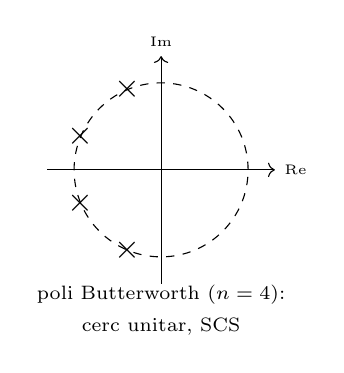
\begin{tikzpicture}[scale=0.85]
\draw[->] (-1.7,0) -- (1.7,0) node[right]{\tiny Re};
\draw[->] (0,-1.7) -- (0,1.7) node[above]{\tiny Im};
\draw[dashed] (0,0) circle (1.3);
\foreach \k in {1,...,4}{
  \pgfmathsetmacro{\ang}{180*(2*\k+3)/8}
  \node at ({1.3*cos(\ang)},{1.3*sin(\ang)}) {\large $\times$};
}
\node[align=center] at (0,-2.1) {\scriptsize poli Butterworth ($n=4$):\\\scriptsize cerc unitar, SCS};
\end{tikzpicture}
\end{center}

\textbf{Exemplu rezolvat:} specificații $\hat G_p=-2$dB la $\omega_p=10$, $\hat G_s=-20$dB la $\omega_s=20$.
$$n=\dfrac{\lg\left[(10^{2/10}-1)/(10^{20/10}-1)\right]}{2\lg(10/20)}=3{,}701 \;\Rightarrow\; n=4$$
$$\omega_c=\dfrac{\omega_p}{\left[10^{-\hat G_p/10}-1\right]^{1/(2n)}}=10{,}693$$
Din tabel, $G^N(s)=\dfrac{1}{s^4+2{,}6131s^3+3{,}4142s^2+2{,}6131s+1}$; înlocuind $s\to s/\omega_c$:
$$G(s)=\dfrac{13073{,}7}{s^4+27{,}942s^3+390{,}4s^2+3194{,}88s+13073{,}7}=\dfrac{13073{,}7}{(s^2+8{,}1844s+114{,}34)(s^2+19{,}758s+114{,}34)}$$

\section*{9. Filtre Chebyshev}
\textbf{Relația de definiție} (filtru TJ normalizat, ordin $n$):
\begin{keyeq}\color{red!65!black}
$$|G^N(j\omega)|=\dfrac{1}{\sqrt{1+\varepsilon^2 C_n^2(\omega)}}\qquad C_n(\omega)=\cos(n\arccos\omega)\quad(\text{polinom Chebyshev})$$
\end{keyeq}
\textbf{Notații/rol:}
\begin{itemize}
\item $C_n(\omega)$ — polinom Chebyshev, recurență $C_n=2\omega C_{n-1}-C_{n-2}$, $C_0=1$, $C_1=\omega$
\item $\varepsilon$ — controlează amplitudinea ondulației (riplului) din banda de trecere; raport câștig max/min $r=\sqrt{1+\varepsilon^2}$, $\hat r[\mathrm{dB}]=10\lg(1+\varepsilon^2)$
\end{itemize}
\textbf{Caracteristica modul-pulsație — proprietăți:}
\begin{itemize}
\item \textbf{ondulații (ripluri) de amplitudine egală} în banda de trecere $0\le\omega\le1$ ($n$ maxime+minime); banda de oprire este netedă (monotonă)
\item la $\omega=1$ modulul $=1/\sqrt{1+\varepsilon^2}$ pentru orice $n$; pentru $\omega>1$ descrește monoton
\item câștig la $\omega=0$: $=1$ dacă $n$ impar, $=1/\sqrt{1+\varepsilon^2}$ dacă $n$ par
\item bandă de tranziție mai mică decât la Butterworth de același ordin, dar cu deteriorarea răspunsului din banda de trecere (apar ripluri)
\item polii sunt plasați pe o \textbf{semielipsă} în SCS (nu pe cerc ca la Butterworth)
\end{itemize}
\textbf{Ordinul $n$:}
\begin{keyeq}\color{red!65!black}
$$n=\dfrac{1}{\cosh^{-1}(\omega_s/\omega_p)}\cosh^{-1}\!\left[\dfrac{10^{-\hat G_s/10}-1}{10^{-\hat r/10}-1}\right]^{1/2}\quad\text{(se rotunjește la întregul superior)}$$
\end{keyeq}

\textit{Notă:} există și varianta \textbf{Chebyshev inversă (FCI)} — răspuns neted (monoton) în banda de trecere și ondulații în banda de oprire (invers față de FC normal); bandă de tranziție cea mai mică dintre toate.

\begin{center}
\begin{tikzpicture}
\begin{axis}[width=7.3cm,height=5cm,xlabel={\scriptsize $\omega$},ylabel={\scriptsize $|G^N(j\omega)|$},xmin=0,xmax=2,ymin=0,ymax=1.05,
  tick label style={font=\tiny}, label style={font=\scriptsize}]
\addplot[thick,purple] table {figdata/cheby_n4.dat};
\draw[dashed] (axis cs:0,0.794) -- (axis cs:2,0.794);
\draw[dashed] (axis cs:1,0) -- (axis cs:1,1.05);
\end{axis}
\end{tikzpicture}\hfill
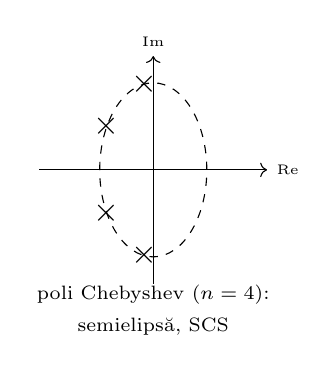
\begin{tikzpicture}[scale=0.85]
\draw[->] (-1.7,0) -- (1.7,0) node[right]{\tiny Re};
\draw[->] (0,-1.7) -- (0,1.7) node[above]{\tiny Im};
\draw[dashed] (0,0) ellipse (0.8 and 1.3);
\foreach \th in {100,150,210,260}{
  \node at ({0.8*cos(\th)},{1.3*sin(\th)}) {\large $\times$};
}
\node[align=center] at (0,-2.1) {\scriptsize poli Chebyshev ($n=4$):\\\scriptsize semielipsă, SCS};
\end{tikzpicture}
\end{center}
\textit{Exemplu numeric din figură:} $n=4$, $\hat r=2$dB ($\varepsilon=0{,}765$) — riplu vizibil sub linia $0{,}794$ în banda $[0,1]$, descreștere monotonă pentru $\omega>1$.

\textbf{Exemplu rezolvat:} specificații $\hat r\le2$dB pentru $0\le\omega\le10=\omega_p$, $\hat G_s\le-20$dB pentru $\omega\ge16{,}5=\omega_s$.
$$n=\dfrac{1}{\cosh^{-1}(1{,}65)}\cosh^{-1}\!\left[\dfrac{10^{2}-1}{10^{0,2}-1}\right]^{1/2}=2{,}99 \;\Rightarrow\; n=3$$
Din tabel (pentru $\hat r=2$dB), $G^N(s)=\dfrac{0{,}3269}{s^3+0{,}7378s^2+1{,}0222s+0{,}3269}$; cu $\omega_p=10$ (înlocuind $s\to s/10$):
$$G(s)=\dfrac{326{,}9}{s^3+7{,}378s^2+102{,}22s+326{,}9}$$

\section*{10. Transformări de frecvență}
Se proiectează întotdeauna mai întâi un filtru \textbf{prototip trece-jos} $H_p(s)$ (Butterworth/Chebyshev/etc.), apoi se înlocuiește $s$ cu o transformare $T(s)$ pentru a obține filtrul dorit:

\begin{keyeq}\color{red!65!black}
\begin{itemize}
\item \textbf{TJ$\to$TS}: $T(s)=\dfrac{\omega_p}{s}$
\item \textbf{TJ$\to$TB}: $T(s)=\dfrac{s^2+\omega_{p1}\omega_{p2}}{(\omega_{p2}-\omega_{p1})s}$
\item \textbf{TJ$\to$OB}: $T(s)=\dfrac{(\omega_{p2}-\omega_{p1})s}{s^2+\omega_{p1}\omega_{p2}}$
\end{itemize}
\end{keyeq}

\textbf{Pași generali (exemplu numeric tip):}
\begin{enumerate}
\item se determină $\omega_s'$ (pulsația de oprire a prototipului) — la TB/OB se alege minimul a două rapoarte (vezi formulele cu $\omega_{p1},\omega_{p2},\omega_{s1},\omega_{s2}$)
\item se determină ordinul $n$ al prototipului TJ (formula de la Butterworth/Chebyshev, cu $\omega_p'=1$, $\omega_s'$ calculat)
\item se determină funcția de transfer normalizată $H(s)$ a prototipului (din tabel)
\item (doar Butterworth) se determină $\omega_c$ și se denormalizează: $H_p(s)=H(s/\omega_c)$
\item se înlocuiește $s\to T(s)$ în $H_p(s)$ pentru a obține funcția de transfer finală $H(s)$ a filtrului dorit
\end{enumerate}

\textbf{Exemplu rezolvat (TJ$\to$TS):} se dorește un filtru \textbf{trece-sus} Chebyshev cu $\omega_s=100$, $\omega_p=165$, $\hat G_s=-20$dB, $\hat G_p=-2$dB.

\textit{Pasul 1 — prototipul TJ:} $\omega_p'=1$, $\omega_s'=\omega_p/\omega_s=165/100=1{,}65$ — exact specificațiile exemplului Chebyshev rezolvat mai sus, deci se reutilizează:
$$H_p(s)=\dfrac{0{,}3269}{s^3+0{,}7378s^2+1{,}0222s+0{,}3269}$$
\textit{Pasul 2 — transformarea TJ$\to$TS:} $T(s)=\omega_p/s=165/s$; se înlocuiește $s\to165/s$ în $H_p(s)$:
$$H(s)=\dfrac{0{,}3269}{\left(\frac{165}{s}\right)^3+0{,}7378\left(\frac{165}{s}\right)^2+1{,}0222\left(\frac{165}{s}\right)+0{,}3269}=\dfrac{s^3}{s^3+515{,}94s^2+61445{,}75s+13742005}$$
Verificare tip: $H(0)=0$, $H(\infty)\to1$ $\Rightarrow$ confirmă \textbf{trece-sus}.

\section*{11. Eșantionarea}
\textbf{Modelarea matematică} — eșantionarea ideală cu un tren de impulsuri Dirac unitare:
$$\delta_{T_e}(t)=\sum_{k=-\infty}^{\infty}\delta(t-kT_e) \qquad x_e(t)=x(t)\,\delta_{T_e}(t)=\sum_{k=-\infty}^{\infty}x(kT_e)\,\delta(t-kT_e)$$
Dezvoltând $\delta_{T_e}(t)$ în serie Fourier complexă ($c_n=1/T_e$) și aplicând TF rezultă \textbf{spectrul semnalului eșantionat}:
$$X_e(\omega)=\dfrac{1}{T_e}\sum_{k=-\infty}^{\infty}X(\omega-k\omega_e), \qquad \omega_e=\dfrac{2\pi}{T_e}$$
adică spectrul semnalului eșantionat este format dintr-o infinitate de replici ale spectrului semnalului continuu, ponderate cu $1/T_e$ și centrate pe multiplii pulsației de eșantionare $\omega_e$.

\textbf{Fenomenul de aliasing:} fie $\omega_m$ = pulsația maximă din spectrul semnalului continuu.
\begin{itemize}
\item dacă $\omega_m<\omega_e/2$ — replicile spectrale nu se suprapun, spectrul original se poate reface exact printr-un FTJ ideal cu banda $[0,\omega_e/2]$
\item dacă $\omega_m>\omega_e/2$ — replicile se suprapun (\textbf{aliasing}), informația se pierde ireversibil, reconstrucția prin FTJ este eronată
\end{itemize}

\textbf{Teorema lui Shannon:} semnalul se poate reconstitui exact din eșantioane dacă pulsația de eșantionare este cel puțin dublul pulsației maxime din semnal:
\begin{keyeq}\color{red!65!black}
$$\omega_e>2\omega_m \quad\text{sau}\quad T_e<\dfrac{T_m}{2}$$
\end{keyeq}
În practică se recomandă o marjă mult mai mare: $\omega_e>10\,\omega_m$.

\begin{center}
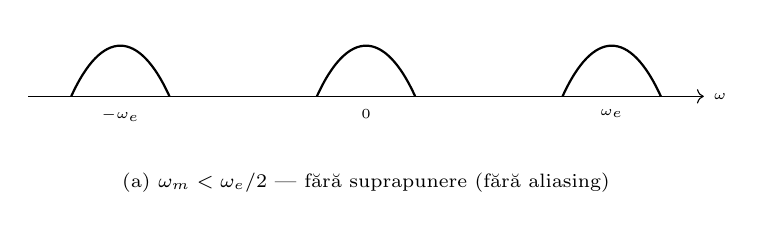
\begin{tikzpicture}[scale=0.78]
\foreach \c/\lbl in {-4/{-\omega_e},0/{0},4/{\omega_e}}{
  \draw[thick] (\c-0.8,0) .. controls (\c-0.3,1.1) and (\c+0.3,1.1) .. (\c+0.8,0);
  \node[below] at (\c,-0.05) {\tiny $\lbl$};
}
\draw[->] (-5.5,0) -- (5.5,0) node[right]{\tiny $\omega$};
\node at (0,-1.4) {\scriptsize (a) $\omega_m<\omega_e/2$ — fără suprapunere (fără aliasing)};
\end{tikzpicture}

\vspace{3mm}

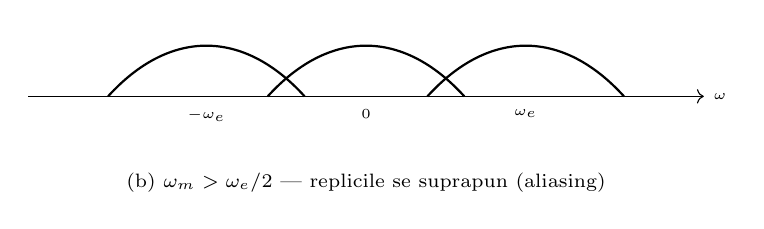
\begin{tikzpicture}[scale=0.78]
\foreach \c/\lbl in {-2.6/{-\omega_e},0/{0},2.6/{\omega_e}}{
  \draw[thick] (\c-1.6,0) .. controls (\c-0.6,1.1) and (\c+0.6,1.1) .. (\c+1.6,0);
  \node[below] at (\c,-0.05) {\tiny $\lbl$};
}
\draw[->] (-5.5,0) -- (5.5,0) node[right]{\tiny $\omega$};
\node at (0,-1.4) {\scriptsize (b) $\omega_m>\omega_e/2$ — replicile se suprapun (aliasing)};
\end{tikzpicture}
\end{center}

\section*{12. Filtre discrete}
\textbf{Forma generală a ecuației cu diferențe} (ordin $n$ recursiv, $m$ nerecursiv):
\begin{keyeq}\color{red!65!black}
$$y[k]=-a_1y[k-1]-\dots-a_ny[k-n]+b_0u[k]+b_1u[k-1]+\dots+b_mu[k-m]$$
\end{keyeq}
echivalentă cu funcția de transfer $z$: $G(z)=\dfrac{b_0+b_1z^{-1}+\dots+b_mz^{-m}}{1+a_1z^{-1}+\dots+a_nz^{-n}}$.

\textbf{Filtre recursive:} cel puțin un coeficient $a_i$ ($i=\overline{1,n}$) este nenul $\Rightarrow$ ieșirea curentă depinde de eșantioane anterioare ale \textbf{ieșirii} (calcul iterativ/recursiv). Răspunsul la impuls Dirac nu se anulează (continuă/se autopropagă) $\Rightarrow$ se mai numesc filtre cu \textbf{răspuns infinit la impuls (IIR)}.

\textbf{Filtre nerecursive:} toți coeficienții $a_i=0$ $\Rightarrow$ ecuația cu diferențe devine $y[k]=b_0u[k]+b_1u[k-1]+\dots+b_mu[k-m]$ — ieșirea depinde \textbf{doar} de eșantioanele intrării (curente și anterioare), nu de ieșiri anterioare. Răspunsul la impuls Dirac se anulează după $m$ eșantioane $\Rightarrow$ se mai numesc filtre cu \textbf{răspuns finit la impuls (FIR)}. Avantaj: pot avea fază riguros liniară (FIR pot, recursive doar aproximativ).

\section*{13. Rezolvare bilete 3 \& 4 — fișă rapidă (răspunsuri punctuale)}

\textbf{Sub. 1 (identic la ambele bilete) — Relațiile de definiție TF/TF$^{-1}$; ce reprezintă spectrul:}
\begin{keyeq}\color{red!65!black}
$$X(\omega)=\int_{-\infty}^{\infty}x(t)e^{-j\omega t}dt \qquad x(t)=\frac{1}{2\pi}\int_{-\infty}^{\infty}X(\omega)e^{j\omega t}d\omega$$
\end{keyeq}
Spectrul Fourier = reprezentarea semnalului în domeniul amplitudine-fază–pulsație; aceeași informație ca reprezentarea temporală, dar arată cum se distribuie amplitudinea/faza pe componentele de frecvență.

\textbf{Sub. 3 — influența unui pol/zero asupra modulului:} caz $-\alpha\pm j\omega_0$, $d$ = distanța de la $j\omega$ curent la pol/zero.
\begin{keyeq}\color{red!65!black}
\textbf{Bilet 3 (zero):} câștigul \textbf{scade} în jurul lui $\omega_0$ (adâncitură); zero exact pe axa $j\omega$ ($\alpha=0$) $\Rightarrow$ câștig \textbf{nul} la $\omega_0$ (notch); fază: $0\to+\pi$.

\textbf{Bilet 4 (pol):} câștigul \textbf{crește} în jurul lui $\omega_0$ (vârf de rezonanță, $|G|=k/d$); $\alpha$ mai mic (pol mai apropiat de axă) $\Rightarrow$ vârf mai mare, la limită $\alpha=0\Rightarrow\infty$; fază: $0\to-\pi$.
\end{keyeq}

\textbf{Sub. 4 — date de proiectare:}
\begin{keyeq}\color{red!65!black}
\textbf{Bilet 3 (trece-bandă):} oprire $[0,\omega_{s1}]\cup[\omega_{s2},\infty)$, trecere $[\omega_{p1},\omega_{p2}]$, cu $\omega_{s1}<\omega_{p1}<\omega_{p2}<\omega_{s2}$.

\textbf{Bilet 4:} trece-sus = \textbf{invers} TJ (oprire $[0,\omega_s]$, trecere $[\omega_p,\infty)$, $\omega_s<\omega_p$); oprește-bandă = \textbf{invers} TB (trecere $[0,\omega_{p1}]\cup[\omega_{p2},\infty)$, oprire $[\omega_{s1},\omega_{s2}]$, $\omega_{p1}<\omega_{s1}<\omega_{s2}<\omega_{p2}$).

Comun: bandă trecere = câștig între $1$ și $G_p$; bandă oprire = câștig sub $G_s$.
\end{keyeq}

\textbf{Sub. 6 — definiție, notații, caracteristica modul-pulsație:}
\begin{keyeq}\color{red!65!black}
\textbf{Bilet 3 (Chebyshev):} $|G^N(j\omega)|=\dfrac{1}{\sqrt{1+\varepsilon^2C_n^2(\omega)}}$, $C_n(\omega)=\cos(n\arccos\omega)$ (polinom Chebyshev), $\varepsilon\to$ riplu. \textbf{Proprietăți:} ondulații de amplitudine egală în BT $[0,1]$, BO monotonă; la $\omega=1$: modul$=1/\sqrt{1+\varepsilon^2}$ pt. orice $n$; la $\omega=0$: $=1$ dacă $n$ impar, $=1/\sqrt{1+\varepsilon^2}$ dacă $n$ par; poli pe \textbf{semielipsă} în SCS.

\textbf{Bilet 4 (Butterworth):} $|G(j\omega)|=\dfrac{1}{\sqrt{1+(\omega/\omega_c)^{2n}}}$. \textbf{Proprietăți:} descrește monoton; câștig$=1$ la $\omega=0$ și $=0{,}707$ ($-3$dB) la $\omega=\omega_c$ \textbf{indiferent de $n$}; poli pe \textbf{cerc unitar} în SCS, separați prin $\pi/n$.
\end{keyeq}

\textbf{Sub. 8 (identic la ambele) — aliasing, teorema eșantionării/Shannon:}
\begin{keyeq}\color{red!65!black}
$$X_e(\omega)=\frac{1}{T_e}\sum_{k=-\infty}^{\infty}X(\omega-k\omega_e)$$
Dacă $\omega_m<\omega_e/2$: replicile nu se suprapun, semnal recuperabil exact prin FTJ ideal. Dacă $\omega_m>\omega_e/2$: replicile se suprapun (\textbf{aliasing}), informație pierdută ireversibil.
$$\textbf{Shannon: } \omega_e>2\omega_m \;\;(\text{practic } \omega_e>10\,\omega_m)$$
\end{keyeq}

\textbf{Sub. 9 — forma generală a ecuației cu diferențe:}
\begin{keyeq}\color{red!65!black}
$$y[k]=-a_1y[k-1]-\dots-a_ny[k-n]+b_0u[k]+\dots+b_mu[k-m]$$
\textbf{Bilet 3 (nerecursive):} toți $a_i=0$ $\Rightarrow$ $y[k]$ depinde \textbf{doar} de intrare $\Rightarrow$ răspuns \textbf{finit} la impuls (\textbf{FIR}); pot avea fază riguros liniară.

\textbf{Bilet 4 (recursive):} cel puțin un $a_i\ne0$ $\Rightarrow$ $y[k]$ depinde și de \textbf{ieșiri anterioare} (calcul iterativ) $\Rightarrow$ răspuns \textbf{infinit} la impuls (\textbf{IIR}).
\end{keyeq}

\textbf{Sub. 2 (identic la ambele bilete) — Filtre: definiția, prototipuri, caracteristici ideale:} definiția + caracteristicile ideale → secțiunea 4.
\begin{keyeq}\color{red!65!black}
\textbf{Prototipuri:} \textbf{Butterworth} (monoton, plat maximal), \textbf{Chebyshev} (riplu în BT, monoton în BO) — și varianta inversă FCI (monoton în BT, riplu în BO), \textbf{eliptic/Cauer} (riplu în ambele benzi, tranziție cea mai abruptă).
\end{keyeq}

\textbf{Sub. 5 — funcția de transfer a circuitului din figură:} ambele circuite sunt cazuri particulare ale tiparelor RLC de la secțiunea 7.
\begin{keyeq}\color{red!65!black}
\textbf{Bilet 3} ($R$ serie, apoi $L$ serie cu $C$ pe ramura de derivație spre masă, $U_o$ luat pe ramura $LC$):
$$H(s)=\dfrac{s^2+\frac{1}{LC}}{s^2+\frac{R}{L}s+\frac{1}{LC}}$$
$H(0)=1$, $H(\infty)=1$, zero pe $j\omega_0$ ($\omega_0=1/\sqrt{LC}$) $\Rightarrow$ \textbf{oprește-bandă} (notch).

\textbf{Bilet 4} ($sL$ serie cu $1/(sC)$ pe ramura serie, apoi $R$ pe derivație spre masă, $U_o$ luat pe $R$):
$$H(s)=\dfrac{\frac{R}{L}s}{s^2+\frac{R}{L}s+\frac{1}{LC}}$$
$H(0)=0$, $H(\infty)=0$, maxim pe $\omega_0=1/\sqrt{LC}$ $\Rightarrow$ \textbf{trece-bandă}.
\end{keyeq}

\textbf{Sub. 7 — funcția de transfer cu specificațiile date (prototip deja dat în enunț):} pasul necesar e \textbf{unic}: substituția $s\to T(s)$ (secțiunea 10), folosind \textbf{doar} $\omega_{p1},\omega_{p2}$. $\omega_{s1},\omega_{s2},G_p,G_s$ \textbf{nu mai intervin} — au fost deja folosite (în alt enunț) ca să se determine ordinul și prototipul, care aici e dat direct.
\begin{keyeq}\color{red!65!black}
\textbf{Bilet 3 (trece-bandă)}: $\omega_{p1}=12,\ \omega_{p2}=26\Rightarrow T(s)=\dfrac{s^2+312}{14s}$; cu $H_p(s)=\dfrac{1}{s^2+1{,}5s+1}$:
$$H(s)=\dfrac{196\,s^2}{s^4+21s^3+820s^2+6552s+97344}$$

\textbf{Bilet 4 (oprește-bandă)}: $\omega_{p1}=5,\ \omega_{p2}=20\Rightarrow T(s)=\dfrac{15s}{s^2+100}$; cu $H_p(s)=\dfrac{1}{(s+1)^2}$:
$$H(s)=\dfrac{(s^2+100)^2}{(s^2+15s+100)^2}$$
\end{keyeq}

\end{document}
